
\section{Motivating example}
\label{sec:mot_example}

Let us consider an analytics task that mines influential reviews
within the click-stream of an e-commerce website consisting of events of type
``Search''(S), ``Read review''(R) and ``Purchase''(P).
The mining task is described in terms of the pattern SR*P, with each event 
variable annotated by its own guard:
\begin{align*}
\text{{\bf S}} \in \Ev&: \facc{S}{name} = ``S"
\\
\text{{\bf R}} \in \Ev&: (\facc{R}{user} = \facc{S}{user} \rightarrow
                          \facc{R}{name} = ``R")
\\
\text{{\bf P}} \in \Ev&: (\facc{P}{name} = ``P") . 
                         (\facc{P}{user} = \facc{S}{user}) . 
                         (\facc{P}{t} < \facc{S}{t} + t_{out}),
\end{align*}
where we consider as input an $\Ev$(name, t, user) relation with fields for 
event name, event timestamp and associated user id, and we use $.$ as a 
shorthand for the conjunctive operator. 
The pattern is described in terms of both selection predicates (for identifying 
the name of the event to be matched), as well as join predicates that make sure 
that the matched events are correlated by the id of the user that performed 
them and that the ``Purchase'' event occurs within a timeout $t_{out}$ from the 
``Search'' event. 
In addition, figure~\ref{fig:srp_pattern} presents the symbolic automata 
representation of the pattern, i.e.\ the state machine where each transition 
has an associated event variable and a corresponding guard.
 

The typical execution plan of this task on a map-reduce framework is to first
group all events by user id, then sort them on time and finally run a pattern
matching engine to detect the desired sequence of events.
In this work we propose to greatly expand the array of possible execution plans
by taking advantage of the fact that a large class of patterns can be
equivalently expressed as SQL queries.
By doing so then one can leverage decades of progress in query optimization to
come up with more efficient query plans than the one outlined above.
For instance, one can express our example pattern as a SQL query as follows:
{\small
\begin{verbatim}
SELECT S.time, P.time, S.user
FROM Ev S, Ev P
WHERE S.time < P.time
AND S.name == "S"   
AND P.name == "P" AND P.time < S.time + t_out
AND P.user == S.user
AND NOT EXISTS ( 
  SELECT * FROM Ev R
  WHERE S.time < R.time AND R.time < P.time
  AND R.user == S.user
  AND R.name != "R"); 
\end{verbatim}
}

The first part of the query enforces the fact that a successful match consists
of an event S followed within a timeout $t_{out}$ by an event P from the same 
user,
while the second part captures the fact that only R events are allowed to take
place in between these two events.
The final result of the query is a set of tuples, one per successful match,
consisting of the timestamps of the initial and final event
in the match and their user id.

Since the number of purchase events P are bound to be much lower than the
search or read review events, performing a broadcast join wrt.\ to the P events
might prove to be the optimum execution plan for this pattern. We remark that
once expressed as an SQL query such optimizations opportunities are dramatically
easier to explore.



The class of patterns that we can currently translate into SQL are those whose
symbolic automata have only cycles of constant length, ie. every repetition
within a particular cycle should consist of the same number of events. 
We note that this class includes the overwhelming majority of patterns discussed
in the literature of complex event processing systems as well as encountered
within an industrial benchmark.

While we acknowledge that for patterns with many transitions, whose
corresponding queries involve many joins, the optimizer might find optimal the
standard query plan based on the pattern matching engine,
we argue that even in such cases one can still leverage the derived query to
minimize the number of events that get grouped by and sorted before being fed to
the pattern matching engine.
Ideally, only the events that will end up as part of a successful match should
undergo this process.
In the following we discuss our approach for performing this pre-processing step
in a time and space efficient manner.


We start by defining for each event variable $X$ of the pattern a 
{\em symbolic set} $\syms{X}$, which collects the values of $X$'s fields that 
are joined by the query, based on the input events matching its selection 
predicates.
\begin{align*}
\syms{S} 
&\coloneq 
\{ \tuple{\facc{S}{t}, \facc{S}{user}} \mid 
S \in \Ev: \facc{S}{name} = \text{``S''}
\}
\\
\syms{\oR} 
&\coloneq 
\{ \tuple{\facc{R}{t}, \facc{R}{user}} \mid 
R \in \Ev: \facc{R}{name} \neq \text{``R''}
\}
\\
\syms{P} 
&\coloneq 
\{ \tuple{\facc{P}{t}, \facc{P}{user}} \mid 
P \in \Ev: \facc{P}{name} = \text{``P''}
\}
\end{align*}
We then re-write the query (using comprehension syntax):
\begin{align*}
&
Q \coloneq 
\{ \tuple{\facc{\symv{s}}{t}, \facc{\symv{p}}{t}, \facc{\symv{s}}{user}} \mid 
\symv{s} \in \syms{S},
\symv{p} \in \syms{P}: \phi(\symv{s},\symv{p}) \}
\\ 
&
\phi(\symv{s},\symv{p}) \equiv 
(\facc{\symv{s}}{t} < \facc{\symv{p}}{t}).\  
(\facc{\symv{p}}{t} < \facc{\symv{s}}{t} + t_{out}).\ 
(\facc{\symv{p}}{user} = \facc{\symv{s}}{user}).\ 
\\
&\qqquad
\slice{\syms{\oR}}
      {(\facc{\symv{s}}{t}\,:\,\facc{\symv{p}}{t}),\; \facc{\symv{s}}{user}} 
= \emptyset  
\end{align*}
where 
$\slice{\syms{\oR}}
       {(\facc{\symv{s}}{t}\,:\,\facc{\symv{p}}{t}),\; \facc{\symv{s}}{user}}$
denotes the slicing of $\syms{\oR}$ defined as:
\begin{align*}
\{ \tuple{ \facc{\symv{r}}{t}, \facc{\symv{r}}{user}} \mid 
\symv{r} \in \syms{\oR} : 
\facc{\symv{r}}{t} \in (\facc{\symv{s}}{t} : \facc{\symv{p}}{t}) .\ 
\facc{\symv{r}}{user} = \facc{\symv{s}}{user}
\},
\end{align*}
which allows us to re-write the \texttt{NOT EXISTS} sub-clause as an emptiness 
test.



\begin{figure}[t]
	\centering
	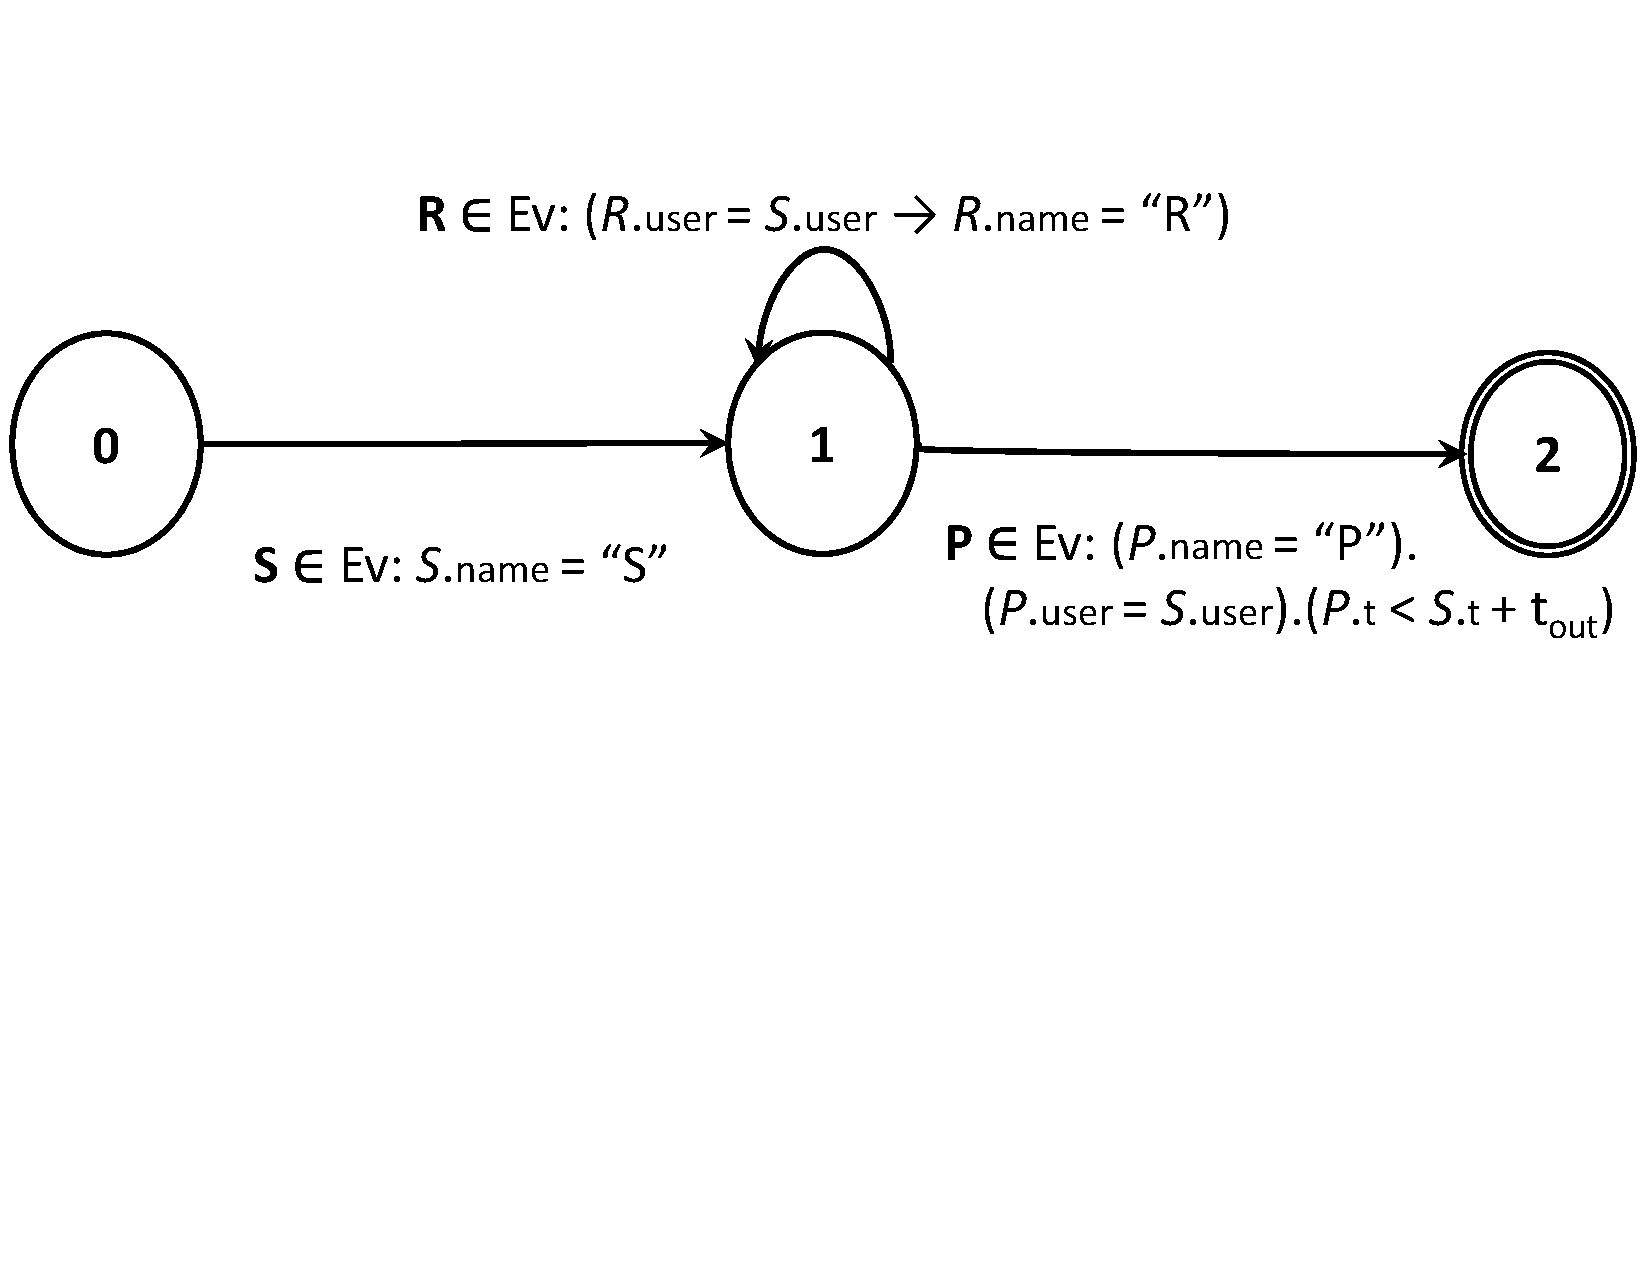
\includegraphics[clip, trim=0cm 10cm 0cm 3cm,width=\columnwidth]
	{graphs/example_sm2.pdf}
	\caption{Symbolic automata for the SR*P pattern.}
	\label{fig:srp_pattern}
\end{figure}



Towards our goal of removing events from the input that are guaranteed not to
participate in a successful match,
% and as such minimize the number of events being sorted and considered by the 
% pattern matcher, 
we generate a {\em precise filter} for each variable in the pattern, that takes 
into account the constraints imposed by the join predicates referencing that 
variable. 
For our example pattern we get the following filters:
\begin{align*}
\precs{S}(\symv{s}) 
&\equiv  
\exists \tuple{\facc{\symv{p}}{t}, \_} \in 
\slice{\syms{P}}
      {(\facc{\symv{s}}{t}\,:\,\facc{\symv{s}}{t} + t_{out}),
       \facc{\symv{s}}{user}} :\ 
\\
&\qquad
\slice{\syms{\oR}}
      {(\facc{\symv{s}}{t}\,:\,\facc{\symv{p}}{t}),\; \facc{\symv{s}}{user}}
 = \emptyset 
\\
\precs{R}(\symv{r}) 
&\equiv
\slice{Q}
      {(-\infty\,:\,\facc{\symv{r}}{t}), 
       (\facc{\symv{r}}{t}\,:\,\infty), 
       \facc{\symv{r}}{user}} 
\neq \emptyset 
\\
\precs{P}(\symv{p}) 
&\equiv  
\exists \tuple{\facc{\symv{s}}{t}, \_} \in 
\slice{\syms{S}}
      {(\facc{\symv{p}}{t} - t_{out}\,:\,\facc{\symv{p}}{t}),  
       \facc{\symv{p}}{user}} :\
\\
&\qquad
\slice{\syms{\oR}}
      {(\facc{\symv{s}}{t}\,:\,\facc{\symv{p}}{t}),\; \facc{\symv{p}}{user}}
= \emptyset,
\end{align*}
which when applied to their corresponding symbolic set will retain only those 
events that contribute to the output of $Q$. 

Since evaluating these filters would in many cases be as expensive as computing
the complete result $Q$, we use them only as a starting point for deriving a set
of {\em abstract filters}, as a ``relaxed'' version of the 
{\em precise filters}, but that can be applied with low processing and 
communication costs.
We do so by employing a series of {\em data and predicate abstractions} 
that generate conservative versions of the original filters.


\newcommand{\oMS}{\overline{M_S}}
\newcommand{\oPS}{\overline{\precs{S}}}

\newcommand{\NotExistsP}{\ident{NotExistsP}}
\newcommand{\NotPrecedesP}{\oPS}
\newcommand{\NotPrecedesPP}{\overline{\omega_S}}
\newcommand{\NotPrecedesPPP}{\overline{\psi_S}}
\newcommand{\NotPrecedesPPPP}{\overline{\upsilon_S}}


\newcommand{\interval}[1]{\lfloor #1 \rceil}
\newcommand{\uinterval}[1]{\lceil #1 \rfloor}
\newcommand{\hashid}[1]{\# #1}

We showcase our techniques on the filter corresponding to the S event variable,
which we first complement in order to obtain the set of "Search" events that we 
want discarded.
\begin{align*}
\oPS(\symv{s}) 
&\equiv  
\forall \tuple{\facc{\symv{p}}{t}, \_} \in 
\slice{\syms{P}}
{(\facc{\symv{s}}{t}\,:\,\facc{\symv{s}}{t} + t_{out}),
	\facc{\symv{s}}{user}} :\ 
\\
&\qquad
\slice{\syms{\oR}}
{(\facc{\symv{s}}{t}\,:\,\facc{\symv{p}}{t}),\; \facc{\symv{s}}{user}}
\neq \emptyset 
\end{align*}

This filter highlights the fact that we can safely remove all ``S'' events that
do not have only ``R'' events between themselves and every succeeding event
``P'' occurring within a $t_{out}$ window of time.

In order to minimize the cost of filtering we use {\em data abstraction} to 
compute time and space efficient representations of sets $\syms{S}$ and 
$\syms{\oR}$.
For example, one could choose to abstract over time and coarsen timestamps $t$
into time intervals $\interval{t}$. 
Then, the time dimension of sets $\syms{S}$, $\syms{\oR}$ could be efficiently 
encoded and queried as interval maps, i.e.\ bit vectors where each bit 
corresponds to a time interval and a set bit would denote the fact that an 
event has occurred within the corresponding interval.
Using this abstraction the filtering predicate becomes:
\begin{align*}
\oPS^{\interval{t}}(\symv{s}) 
&\equiv  
\forall \tuple{\facc{\symv{p}}{t}, \_} \in 
\slice{\syms{P}}
{\interval{\facc{\symv{s}}{t}\,:\,\facc{\symv{s}}{t} + t_{out}},
	\facc{\symv{s}}{user}} :\ 
\\
&\qquad
\slice{\syms{\oR}}
{\uinterval{\facc{\symv{s}}{t}\,:\,\facc{\symv{p}}{t}},\; 
 \facc{\symv{s}}{user}}
\neq \emptyset 
\end{align*}
where in order to maintain conservativeness (ie.\
$\NotPrecedesP^{\interval{t}} \rightarrow \NotPrecedesP$) we had to
over-approximate the $\facc{\symv{s}}{t}:\facc{\symv{s}}{t} + t_{out}$ 
range, but under-approximate the
$\facc{\symv{s}}{t}:\facc{\symv{p}}{t}$ interval.
Thus, we note that depending on the filter, the data abstractions that we
use must be able to provide both over- and under- approximations of the original
sets. 
  

If on the other hand we abstract over user ids via hashing, that is
use a compact representation of sets $\syms{S}$, $\syms{\oR}$ that stores time
information only per user hash bucket as opposed to individual user ids, then
the resulting symbolic filter:
\begin{align*}
&
\NotPrecedesP^{\hashid{user}}(\symv{s}) \equiv 
\forall\; \tuple{\facc{\symv{p}}{t}, \_} \in 
\slice{\syms{P}}
{(\facc{\symv{s}}{t}\,:\,\facc{\symv{s}}{t} + t_{out}),
	\hashid{\facc{\symv{s}}{user}}} :\ 
\\
&\qqquad\qquad\quad
\slice{\syms{\oR}}
{(\facc{\symv{s}}{t}\,:\,\facc{\symv{p}}{t}),\; 
	\hashid{\facc{\symv{s}}{user}}}
\neq \emptyset 
\end{align*}
does not satisfy our safety requirement 
(i.e.\ $\NotPrecedesP^{\hashid{user}} \nrightarrow \NotPrecedesP$).
This happens because hashing can only provide over-approximations of sets while,
in order to ensure conservativeness, the abstractions used for this filter need
to provide both over and under approximations.
While there are several ways to address this issue (for an alternative solution 
see section~\ref{sec:data_abstraction}), 
in the following we show how {\em predicate abstraction} can alleviate the 
problem.


Predicate abstraction encompasses a set of re-writings 
that strengthen the filter by discarding those constraints that cannot be safely
or efficiently abstracted over.
For instance, our filter could be strengthened into:
\begin{align*}
&
\NotPrecedesPPP(\symv{s}) \equiv 
\slice{\syms{P}}
{(\facc{\symv{s}}{t}\,:\,\facc{\symv{s}}{t} + t_{out}),\; 
	\facc{\symv{s}}{user}}
 = \emptyset,
\end{align*} 
which eliminates only those search events that are not followed by a purchase
event within $t_{out}$, and was obtained from the base case of
the universal quantifier in $\NotPrecedesP$.
Since this version only requires over-approximation, one can safely use hashing
to abstract over the user id dimension of $\syms{P}$, i.e.\ 
$\NotPrecedesPPP^{\hashid{user}} \rightarrow \NotPrecedesPPP$, where
\begin{align*}
&
\NotPrecedesPPP^{\hashid{user}}(\symv{s}) \equiv 
\slice{\syms{P}}
{(\facc{\symv{s}}{t}\,:\,\facc{\symv{s}}{t} + t_{out}),\; 
	\hashid{\facc{\symv{s}}{user}}}
 = \emptyset .
\end{align*}

Moreover, predicate abstraction also reveals the well known Bloom
join algorithm as an instance of our approach, wrt.\ the join
predicate $\facc{P}{user} = \facc{S}{user}$ from the original query. 
This becomes apparent if we ignore time in the filter above:
\begin{align*}
&
\NotPrecedesPPP^{\hashid{user}}(\symv{s}) \equiv 
\slice{\syms{P}}{*, \hashid{\facc{\symv{s}}{user}}}
 = \emptyset,
\end{align*}
and we use a Bloom filter to implement 
$\slice{\syms{P}}{*, \hashid{\facc{\symv{s}}{user}}}$.
More importantly, it highlights the fact that one can use data and predicate 
abstraction to explore the entire spectrum of abstract filters, and make the 
choice between precision vs overheads on a case by case basis.
We discuss additional scenarios where predicate abstraction proves
beneficial in section~\ref{sec:pred_abstraction}.




\begin{comment}
\\
&
\NotExistsP(t_S, user_S) \coloneq 
E_P(t_S..t_S+t_{out}, user_S) = \emptyset

These filters are designed to be applied independently over the input without
the need to perform any joins, group by's or order by's.
More importantly, in a map-reduce framework they can be performed with minimal
communication overhead.


- interval map may use different granularities in different regions of the
timeline, i.e. finer granularity in regions with higher probability of events
\end{comment}





































\section{Design}
\label{sec:design}

We consider queries specified as a symbolic finite automaton where each
transition is annotated by a variable and a guard.
The variable is used to bind the fields of the currently considered event while 
the guard is a propositional formula in disjunctive normal form which decides 
whether the transition can be triggered or not.  
The atomic formulas of the guard are either {\em selection} predicates, which 
only reference the variable associated with the current transition,
or {\em join} predicates, which may also reference the variables of preceding 
transitions.
In particular, the guards of start transitions can only use selection 
predicates.  
   
Pattern matching algorithms require the input stream of events to be
(partially) sorted on time, while this is not always the case in practice due
to competing constraints of other stages in the data processing pipeline. 
Thus, evaluating pattern matching queries in a map-reduce framework usually 
adds a reduction step in order to sort the input, which can become the main 
bottleneck of the analysis, both at the network level (large amounts of 
shuffled data) and at the processing level (in case of data-skew).

The standard approach to minimize the cost of sorting/data shuffling has been 
to introduce a {\em preprocessing} phase which first filters the input based on 
the {\em selection} predicates in the transition guards, i.e.\ removes all 
events that do not satisfy the guard of at least one transition while ignoring 
its {\em join} predicates.
This {\em preprocessing} phase can significantly reduce both processing costs 
and latency since it takes linear time in the size of the input (as opposed to 
$O(nlogn)$ for sorting) and is embarrassingly parallel, i.e.\ scales out with 
the number of computing resources available.
Moreover, it can be merged with the previous operator in the data processing 
pipeline thus incurring no extra costs for materialization or data transfer.    


In our work we extend the opportunities for query plan optimizations across all 
the stages of the workload, beyond just pipelining the preprocessing phase of 
the pattern matcher, by leveraging the fact that a large class of symbolic 
finite automata have a corresponding relational calculus expression (possibly 
with counting quantifiers).
Whenever that is not the case we can narrow the scope of our optimizations to 
the sections of the pattern that do.
The resulting relational expressions can then be optimized within the scope of 
the entire (predominantly relational) workload based on decades of progress in 
relational optimizations.  
We remark that the translation to relational expressions is not limited only to 
acyclic symbolic automata, but also to automata with cycles of fixed length, 
i.e.\ each iteration of the cycle has the same number of transitions.
This class of symbolic automata is of particular importance as it includes the 
vast majority of patterns found in benchmarks and in industrial workloads.  


Even in the scenarios where the relational optimizer decides that using the 
pattern matcher leads to the most efficient query plan, we can leverage the 
relational expressions to generate a series of {\em abstract} filters that can 
dramatically increase the reduction ratio achieved by the preprocessing step by 
also taking advantage of the filtering power of {\em join} predicates (as 
opposed to just the {\em selection} predicates).   
Thus, in many cases we manage to discard most of the events that are guaranteed 
not to take part in a successful match and significantly reduce the amount of 
data fed into the pattern matcher.

We start from the relational formulas and produce {\em symbolic} filters for 
each transition, that retain only those events from the input which trigger 
that transition and take part in a complete match.
However in many cases these filters would be too expensive to build and 
evaluate as such.
Therefore, we coarsen them to obtain a set of {\em abstract} filters
that can be constructed and queried in a time and space efficient manner.
In particular, we make use of both {\em data} abstraction and {\em predicate} 
abstraction in order to generate filters that, while conservative, closely 
match the {\em symbolic} filters. 
We explore the trade-offs between the overheads incurred in building/querying
the filters and their accuracy. 


The derivation of abstract filters is not strictly tied to the ability to 
generate a semantically equivalent relational expression for a symbolic 
automaton. By adding the fixpoint construct, we are able to apply similar 
techniques to generate both the {\em symbolic} and the {\em abstract} 
filters.


\begin{comment}
We propose three levels of abstraction.
The first enforces the join constraints between different transitions as
expressed by join predicates within the transition guards.
The second one further imposes time windowing constraints (all events of a
successful match must occur within a timeout of the first event in the match).
Finally the last one enforces ordering constraints between {\em consecutive}
transitions of the pattern.
\end{comment}

\subsection{From automata to relational expressions}

We assume that patterns are specified in terms of symbolic finite automata and
we formally define a symbolic finite automaton as $\cA = (S, T, s_{start}, C),$ 
where $S$ is the set of states, $T$ is the set of transitions, $s_{start}$ is 
the initial state and $C$ is the set of completion (accepting) states.
Each transition is defined in terms of the tuple $(X, p_X, src, dst)$ where $X$ 
is the variable binding the event considered for that transition, $p_X$ is the 
guard deciding whether the transition is triggered or not, and $src$ and $dst$ 
are the transition's source and destination states.

{\bf Notation.}
We usually denote states by indices $i, j, k,$, and we abuse notation to refer 
to transitions using the variable name they introduce (eg. $X, Y, Z$).
In addition we refer to states and transitions also as nodes and edges, 
respectively, in the corresponding graph of an automaton.

To streamline the presentation we begin by considering automata with only
cycles of length 1 and we distinguish between cycle transitions and
non-cycle transitions.


The translation process produces one relational query $Q_i$ per state $i$, and 
the final relational expression of the automata is obtained by unioning all the 
queries generated for the automata's accepting nodes.
Evaluating query $Q_i$ over a set of events computes partial matches, i.e.\ 
sequences of events, corresponding to all the possible paths between the 
starting node and node $i$.
Therefore, if $i$ is the starting node then its query returns an empty sequence 
while if $i$ is an accepting node then it returns complete matches found in the 
input stream of events.
Moreover, the partial (complete) matches computed by $Q_i$ do not include the 
events matched against cycle transitions therefore have a bounded length. 

The schema of the queries we generate consist of a sequence of event variables, 
one for each non-cycle transition that may occur along its associated set of 
paths. 
If a transition is triggered within a partial match, then its corresponding 
variable is initialized by the event that triggered it, otherwise that variable 
is assigned null.


State queries $Q_i$ are defined as the union of transition queries $Q_X$ over 
all the incoming non-cycle transitions into state $i$, where each transition 
query $Q_X$ computes partial matches corresponding to the paths ending with 
transition $X$.
In turn, the $Q_X$ query corresponding to a non-cycle transition is defined as 
the join between node query $Q_k$ and the input relation of events, where $k$ 
is the source of the transition and each event considered is bound by event 
variable $X$.
The condition enforced by $Q_X$ consists of the guard $p_X$ along with the 
constraint that the timestamp of $X$ succeeds the last event in the partial 
match produced by $Q_k$.
Additionally, a nested query ensures that no other events 
exist between the last event matched by $Q_k$ and the event bound by $X$, 
except for events matching cycle transitions starting and ending in $k$.


The translation process iterates in topological order over the nodes of the DAG
obtained by ignoring the cycle transitions of the automaton.
At each node $i$, it first generates the queries for all its incoming
non-cycle transitions $Q_X$ and then $Q_i$ is defined as their union. 
The schema of $Q_i$ is established as the union of the schemas of the incoming 
transitions $Q_X$.


In order to perform this translation for all automata whose cycles have a fixed 
length ($\geq 1$), we first normalize them such that each cycle starts and ends 
with the same state.
More formally, the cycles of a normalized automata have a single incoming edge 
and a single outgoing edge and both of them enter and exit, respectively, the 
same node.
We remark, that cycles of fixed length cannot have transversal edges (paths), 
i.e.\ edges (paths) that connect non-adjacent nodes, as this would violate the 
restriction that each iteration of the cycle has the same length.

Given an automaton with a cycle that has multiple incoming and outgoing edges 
we first duplicate the cycle for each additional incoming edge. 
Then we duplicate the path between the starting and ending nodes of the cycle, 
where starting node of a cycle is defined as the destination of its incoming 
edge while the ending node is the source of the last of its outgoing edges. 
Finally, we change the source of each outgoing edge to be the corresponding 
node in the newly created path, resulting in a cycle whose incoming and 
outgoing edges have the same node as destination and source, respectively.
By applying this procedure to every cycle with multiple incoming and outgoing 
edges we obtain a normalized automaton.  
We remark that, while the resulting automaton may have multiple cycles starting 
and ending with the same node, all of those must also have the same length.


The only part of the translation process that changes when generalizing from 
automata with single edge cycles to normalized automata is the specification of 
transition queries $Q_X$, and in particular, the specification of its nested 
query should the source state of $X$ be the starting/ending point of a cycle.
We recall that in the case of cycles with a single transition $Y$ the nested 
query enforces that all events occurring in the interval between the last event 
in the partial match computed by $Q_k$ and the timestamp of event variable $X$ 
satisfy guard $p_Y$. 
By contrast, in the case of multi-edge fixed length cycles, for each event in 
the same interval we establish its position (based on  the count of events with 
smaller timestamps) and we ask that it satisfies the guard of the transition 
corresponding to that position in the cycle modulo the length of the cycle.
If multiple cycles initiate and conclude at the same node, we alternatively 
have to enforce that all events in an iteration satisfy the corresponding 
transition guards of a particular cycle.


\subsection{Symbolic filter generation}
\label{sec:prec_filter_generation}



After translating patterns into relational queries a host of relational 
optimizations become applicable, from column pruning and partial aggregation to
the selection of specific join algorithms.
In the following we detail our proposal for speeding up pattern matching in a 
distributed environment based on its representation in the relational world as 
a series of unions and joins.
More specifically, even though this representation may prove too expensive to 
evaluate directly, one can still use it to design filters meant to discard from 
the input (almost) all the events that do not participate in a complete match 
and thus vastly reduce the number of events ultimately processed by the pattern 
matching engine.
 
 % discuss difference between fields referenced by selection predicates and 
 %fields referenced by join predicates, and how the symbolic filters are 
 %concerned with the latter.


The first step in this process is to generate for each transition of the 
automaton a {\em symbolic} filter.
These filters are precise in the sense that they retain only the events  
guaranteed to appear in a successful match.
While it is understood that constructing and applying such filters is 
prohibitively expensive, we discuss them nonetheless as they are essential in 
guiding the design of {\em abstract} filters, their time and space efficient 
variants. 
In current work we derive such filters only for non-cycle transitions and 
single-edge cycles since the filters for transitions in multi-edge cycles 
are impractical to build/apply and abstract over, as they require the position 
of the considered event within a particular time interval.



Given an automaton $\cA$ for which we can derive a semantically equivalent  
relational query $Q_{\cA}$, the symbolic filter $F_X$ corresponding to one of 
its non-cycle transition $X$ is extensionally defined in terms of the events 
from the input that bind the event variable $X$ in the output of $Q_{\cA}$. 
Therefore $F_X$ can be obtained from $Q_{\cA}$ by projecting away (i.e.\ 
existentially quantifying) all the other event variables in its output besides 
$X$.

The symbolic filter $F_Y$ of a cycle transition $Y$, with node $k$ as source 
and destination, selects from the input those events that occur within interval 
$(t_Z, t_W)$, where $t_Z, t_W$, are the timestamps of a pair of event variables 
$Z, W$, from the output of $Q_{\cA}$ such that $Z, W$ are associated to 
non-cycle transitions entering and respectively exiting $k$.
In addition, $F_Y$ also enforces the guard $p_Y$ with its join predicates 
ignored, as they are guaranteed to be satisfied based on the fact that the 
nested query generated as part of the definition of $Q_W$ (and which includes 
$p_Y$) was found to hold during the evaluation of $Q_{\cA}$.

\begin{comment} 
The two kinds of transitions (cycle vs non-cycle) generate distinctly different 
kinds of symbolic filters. 
While both make use of the relational query $Q_{\cA}$ generated for the 
automaton, only the filter for cycle transitions makes direct use of its results
while the other simply uses $Q_{\cA}$'s expression as a starting point for its 
definition.
This distinction plays an important role in how we go about building these 
filters in a distributed environment.
\end{comment}


We take a bottom-up approach to building the symbolic filters as it allows us 
to outline an evaluation strategy that operates over sets and which uses set 
operations like union, intersection, set membership or emptiness testing. 
Adopting such a set-centric evaluation strategy is advantageous in a 
distributed environment due to the embarrassingly parallel nature of many set 
operators, but more importantly it gives us a powerful knob in terms of the set 
representations that we use, such that we can trade off precision in favor of 
performance. 
This strategy is what ultimately guides the design of the {\em abstract} 
filters (which we discuss in sections~\ref{sec:data_abstraction} 
and~\ref{sec:pred_abstraction}) which make our solution practical.
   

As a first step we build for every transition $X$ of an automaton $\cA$ so 
called "symbolic sets", which collect for every event matching the selection 
predicates of $p_X$ those fields of event variable $X$ referenced by join 
predicates throughout all the transition guards of $\cA$.
We then re-write the symbolic filters by replacing each event variable and 
selection predicate associated to a transition with its corresponding symbolic 
set.
Finally, the join predicates get re-written in terms of slicing, intersection 
and emptiness testing over these sets.


\subsection{Data abstraction}
\label{sec:data_abstraction}


Building the symbolic filters as described in the previous section is not a 
feasible option, as it would require at least just as much work as computing 
the final result.
Nonetheless, the symbolic filters provide an excellent template for designing 
appropriate set abstractions that can provide the set operations required for 
their constructing and querying them in a time and space efficient manner. 
Our approach is to use set abstractions that sacrifice precision, while 
remaining conservative, as we should never eliminate events that would 
otherwise have contributed to a successful match.
We call the resulting structures {\em abstract} filters as they are the outcome 
of employing several abstractions during the process outlined for deriving the 
symbolic filters.  


First of all, we remark that the sets we abstract over contain tuples as 
opposed to single values, where each tuple field holds the values relevant to a 
particular join predicate. 
Similarly, the abstractions we chose need to be multidimensional in the sense 
that they must allow the testing of the domain of values corresponding to a 
specific join predicate, independent of the others.  
Second, we note that besides supporting set intersection and set union, the 
choice for a particular set abstraction is deeply influenced by the particular 
kind of predicates said abstractions needs to support.
For example, in the case of equality joins an appropriate data abstraction 
would be to use bloom filters as they provide a low cost solution for testing 
whether o value belongs to a set, with the guarantee of no false negatives.
For enforcing inequality joins on the other hand, an interval map, i.e.\ a 
bit vector where each bit stands for a particular interval in the domain,
provides a similarly low cost abstraction.  

\begin{example}
One way to address the issues raised by hash-based data abstraction is to 
re-write the precise filter using min aggregates:
\begin{align*}
&
\NotPrecedesPP(\symv{s}) \equiv 
\min \{ 
\facc{\symv{r}}{t} \mid 
\tuple{\facc{\symv{r}}{t}, \_} \in 
\slice{\syms{\oR}}
{(\facc{\symv{s}}{t}\,:\,\facc{\symv{s}}{t} + t_{out}),\; 
	\facc{\symv{s}}{user}} 
\}
\\
&\qquad
< \min \{ 
\facc{\symv{p}}{t} \mid 
\tuple{\facc{\symv{p}}{t}, \_} \in 
\slice{\syms{P}}
{(\facc{\symv{s}}{t}\,:\,\facc{\symv{s}}{t} + t_{out}),\; 
	\facc{\symv{s}}{user}}
\}.
\end{align*}
Now, we can safely use hashing to abstract over user ids based on the following
symbolic filter:
\begin{align*}
&
\NotPrecedesPP^{\hashid{user}}(\symv{s}) \equiv 
\\
&\qquad
\max_{u \in \hashid{user_S}}
\min \{ 
\facc{\symv{r}}{t} \mid 
\tuple{\facc{\symv{r}}{t}, \_} \in 
\slice{\syms{\oR}}
{(\facc{\symv{s}}{t}\,:\,\facc{\symv{s}}{t} + t_{out}),\; 
	u} 
\}
\\
&\qquad
< 
\min_{u \in \hashid{user_S}}
\min \{ 
\facc{\symv{p}}{t} \mid 
\tuple{\facc{\symv{p}}{t}, \_} \in 
\slice{\syms{P}}
{(\facc{\symv{s}}{t}\,:\,\facc{\symv{s}}{t} + t_{out}),\; 
	u}
\}.
\end{align*}
\end{example}
While for our example it was possible to come up with an alternative formulation
of the filter, this may not always be the case. 
And even in the cases where it is, the alternatives may be too expensive to
materialize and query (for eg.\ evaluating $\NotPrecedesPP^{\hashid{user}}$ is
clearly more costly than $\NotPrecedesP^{\interval{t}}$).
Therefore, in the next section we discuss how {\em predicate abstraction} can 
mitigate these kinds of challenges.

\subsection{Predicate abstraction}
\label{sec:pred_abstraction}


We propose {\em predicate abstraction}, ie.\ the technique of strengthening
 the
symbolic filters by discarding some of their predicates, as a way of
 overcoming
the challenges that can arise when turning symbolic filters into abstract 
filters.
For example, it may happen that for some predicate types
(for eg.\ $x.Contains(y)$, where $x$, $y$ are strings) we simply cannot
 provide
any data abstraction, and even for those that we can, materializing and
 querying
those data abstractions might prove too expensive.

Predicate abstraction is an essential component of our approach
allowing us to strike the right balance between the data reduction that the
symbolic filters provide on one hand, and the overheads introduced by their
data abstractions on the other.
For instance, we may choose to discard
predicates that have very low selectivity, i.e.\ the reduction in input 
data
that they provide does not justify the cost of enforcing them.
Similarly, one may turn to predicate abstraction when dealing with patterns
 with
a large number of join predicates or transitions, in order to mitigate the
increased overheads incurred by their data abstractions.

Considering that initial or final transitions typically have the fewest
number of matching events, one might choose to generate filters that only
consider the join predicates with respect to those transitions.
Due to the low cardinality of the sets of events matching these transitions 
the join predicates referencing them are likely to have very high 
selectivity.
Moreover, the data abstractions used to enforce them can achieve higher
precision for the same operating costs.




\subsection{Building filters through fixpoint}


We remark that the symbolic filters are not strictly tied to the ability to 
express automata as relational queries, but that they can also be obtained for 
an arbitrary automaton by using a fixpoint operator that keeps track of 
provenance information.
The fixpoint operator we consider assigns to the starting node the empty 
sequence and then iteratively builds for every node of the automaton its 
corresponding set of (partial) matches, until no more new matches are found. 
In every iteration, for each node $i$ and each of its outgoing transitions $X$, 
the partial matches added by the previous round to $i$ get extended if matching 
events are found within the symbolic set of $X$. 
The newly found matches then get added to the collection of matches 
corresponding to $X$'s destination, and the process starts over.  
Since we never remove partial matches we are guaranteed to reach a fixpoint.
Whenever we add a new match to an accepting node, we also update the symbolic 
filters of the transitions along the path followed by that match.

In designing the fixpoint operator we similarly make extensive use of sets and 
set operators.
In particular, the (partial) matches we compute for each node $i$ of the 
automaton are represented as a series of sets, one for each transition that may 
occur on a path from the start node to $i$.
Then the symbolic filter for a specific transition can be obtained by unioning 
its corresponding set across all the accepting nodes.
When deciding whether a partial match can be extended by triggering transition 
$X$ we simply intersect the symbolic set of $X$ with the projection from the 
partial match of all its fields that are joined in the guard of $X$.
If the result is empty then the extension is not possible, otherwise a new 
partial match gets created whose corresponding set for transition $X$ is the 
result of the intersection.   





 
